\% AUTHOR DATA
\%\%\%\%\%\%\%\%\%\%\%\%\%\%\%\%\%\%\%\%\%\%\%\%\%\%\%\%\%\%\%\%\%\%\%\%\%\%\%\%\%\%\%\%\%\%\%\%\%\%

\rokegz{2019r.}
\rokak{2018/2019}
\semestr{Zima}
\stopien{II}
\kierunek{Informatyka}
\instytut{informatyki}
\jednostka{Instytut Informatyki}
\specjalnosc{Inżynieria Systemów Informatycznych}
\typ{magisterska}
\autor{Bruce Wayne}
\nralbumu{-1}
\adresa{1007 Mountain Drive}
\adresb{Gotham City}
\foto{personal/infocard/portrait.jpeg}
\dataurodzenia{February 2nd, 1974}
\datarozpoczecia{October 1st, 2010}

\% THESIS DATA
\%\%\%\%\%\%\%\%\%\%\%\%\%\%\%\%\%\%\%\%\%\%\%\%\%\%\%\%\%\%\%\%\%\%\%\%\%\%\%\%\%\%\%\%\%\%\%\%\%\%

\opiekun{Lucius Fox PhD}

\tytul{Automatyczny sposób ewaluacji przestępstw}
\tytulen{An automated system of crime evaluation}

\zyciorys{Bruce Wayne podróżuje od 14. roku życia. Ukończył kursy na Sorbonie i innych uniwersytetach europejskich. Nigdy nie pozostał na uczelni na tyle długo by ukończyć semestr, stąd w naukach czy inżynierii nie legitymuje się żadnym tytułem - niemal na pewno zna jednak osobiście ministra edukacji urzędującego w kraju czytelnika. Poza życiem akademickim przyswoił rozmaite sztuki walki w czasie swych licznych podróży oraz opracował szerokie portfolio wynalazków. Spośród tych ostatnich większość pozostaje ściśle tajna jako prywatny majątek rodzinnej korporacji.\\[3mm]
Poniżej podpis:}

\streszczenie{Celem tej pracy jest zaprojektowanie i udostępnienie prototypu rozwiązania problemu zdalnej akwizycji informacji o wzorcach, występujących w danych prawnie klasyfikowanych jako wrażliwe.\\[3mm]
Cel ten motywowany jest minimalizacją powierzchni ataku na dane natury osobistej, a także ograniczeniem kosztów dodatkowej infrastruktury potrzebnej dostawcy do wdrożenia usługi. Proponowany model osiąga to poprzez zaangażowanie odbiorcy, który zyskuje w ten sposób dodatkowe możliwości. W pracy przedstawiono architekturę opracowaną na potrzeby celu szczegółowego w postaci automatycznej certyfikacji elastycznych odbiorców energii elektrycznej.\\[3mm]
Dla osiągnięcia celu użyto autorskich algorytmów zaprojektowanych z użyciem wzorców programowania asynchronicznego i współbieżnego, oraz ich prototypowych implementacji.}

\streszczenieen{The aim of this thesis is design and publication of a prototype of a solution to the problem of remote aquisition of information about patterns emergin in data classified as sensitive by law.\\[3mm]
The mentioned aim is motivated by a vision of lessening the attack surface where data of personal nature is concerned; also - of limiting the cost of additional infrastructure needed by the provider in order to implement the service. The proposed model achieves that through engagement of the user, who in turn gains additional possibilities. In this document an architecture is presented, designed to fulfill a specific purpose of automatizing certification of flexible users of electric energy.\\[3mm]
Used for the purpose of achieving the stated goal were original, customly designed algorithms based on patterns of asynchronous and parallel programming, together with their prototypical implementations.}

\slowakluczowe{DSR, pomiar elastyczności, architektura, programowanie asynchroniczne.}
\slowakluczoween{DSR, flexibility estimation, architecture, asynchronous programming.}

\renewcommand{\passthrough}[1]{#1}

\ifdraft
    \clearpage
    
\includepdf[pages=-]{test/recenzja-nowy-formularz.pdf}
    \section*{Najnowsze zmiany w projekcie}
    \thispagestyle{empty}
\fi

\maketitle
\makeinfo
\makeabstracts

\thispagestyle{empty}
\cleartooddpage
\tableofcontents

\cleartooddpage

\hypertarget{wykaz-skruxf3tuxf3w}{%
\chapter*{Wykaz skrótów}\label{wykaz-skruxf3tuxf3w}}
\addcontentsline{toc}{chapter}{Wykaz skrótów}

\begin{itemize}
\tightlist
\item
  MITM (ang. \emph{man-in-the-middle}) - atak dokonywany przez
  podstawionego pośrednika.
\end{itemize}

\hypertarget{definicje}{%
\chapter*{Definicje}\label{definicje}}
\addcontentsline{toc}{chapter}{Definicje}

\begin{itemize}
\tightlist
\item
  odbiorca - gospodarstwo domowe lub przedsiębiorstwo pobierające
  energię elektryczną,
\item
  agregator - podmiot gromadzący odbiorców celem zaoferowania
  operatorowi sieci przesyłowej zwiększonej stabilności,
\item
  FMA (\emph{Flexibility Measurement Architecture}) - architektura
  pomiaru elastyczności opisywana w niniejszej pracy,
\item
  użytkownik - odbiorca energii korzystający z implementacji
  proponowanej architektury do celów pomiaru własnej elastyczności,
\item
  zamawiający - agregator użytkowników,
\item
  scenariusz - określany przez zamawiającego zbiór warunków, jakie muszą
  zostać spełnione dla zaliczenia użytkownikowi próby elastyczności,
\item
  DSR (\emph{demand-side response}) - program angażowania strony
  popytowej w zapewnienie stabilności sieci elektroenergetycznej,
\item
  elastyczność - zdolność odbiorcy do modyfikowania swego profilu
  zapotrzebowania na żądanie
  {[}\protect\hyperlink{ref-finck_quantifying_2018}{1}{]},
\item
  indeks elastyczności - miara elastyczności oznaczana symbolem \(FI\),
  obliczana przez uśrednienie wag wypełnionych przez użytkownika
  scenariuszy przy zastąpieniu wszystkich scenariuszy nie wypełnionych
  wartością \(0\),
\item
  pomiar elastyczności - proces wyznaczania indeksu elastyczności,
\item
  próba elastyczności - składowa procesu pomiaru elastyczności odbiorcy,
\item
  \(FI\) - wartość spełniająca warunki:
  \(FI = x \vert x \in {\rm I\!R^+} \land x \le 1\)
  {[}\protect\hyperlink{ref-junker_characterizing_2018}{2}{]},
\item
  architektura korporacyjna - architektura opisująca przedsiębiorstwo
  jako system dla celów analizy lub wprowadzenia zmian; wbrew brzmieniu
  terminu nie rozumiemy pod nim jedynie ``korporacji'' w polskim
  znaczeniu tego słowa {[}\protect\hyperlink{ref-leks_pare_2010}{3}{]}.
\end{itemize}

\hypertarget{wstux119p}{%
\chapter{Wstęp}\label{wstux119p}}

W sierpniu 2015 roku polski rynek energii elektrycznej po raz pierwszy
od 35 lat znalazł się w sytuacji wprowadzenia 20 stopnia zasilania
{[}\protect\hyperlink{ref-dolega_national_2018}{4}{]}. Powodem były
przedłużające się susze i związany z nimi niedobór wody niezbędnej do
chłodzenia generatorów w elektrowniach.

Mechanizm stopni zasilania zaprojektowany został właśnie z myślą o
takich sytuacjach. Pozwala on w sytuacji krytycznej unikąć tzw.
\emph{blackoutu} poprzez wprowadzenie czasowych limitów poboru energii
dla podmiotów o zapotrzebowaniu powyżej 300 KW. Limity te są drastyczne
i równe dla wszystkich największych odbiorców. Alternatywą dla
wprowadzenia stopni zasilania pozostaje jedynie wyłączenie zasilania na
całym obszarze, a nagły, gwałtowny wzrost zapotrzebowania na energię
może wystąpić z dnia na dzień
{[}\protect\hyperlink{ref-pap_pse_2015}{5}{]}.

Sposobem na wykorzystanie siły wolnego rynku dla utrzymania zagrożonych
dostaw energii jest program DSR. Według jego założeń, w sytuacji nagłego
niedoboru energii niektóre podmioty dobrowolnie rezygnują z zaspokojenia
części swego zapotrzebowania na rzecz pozostałych podmiotów.
Wstrzymujący się od części konsumpcji otrzymują odpowiednie finansowe
wynagrodzenie, a jego wymiar zależy od wielkości dostawy i jej zgodności
z umową.

Jedną z podstawowych potrzeb programu DSR jest natomiast ocena wartości
strategicznej poszczególnych odbiorców, którzy oceniani są według
możliwości dostosowania własnego zapotrzebowania na energię do warunków
panujących w Krajowej Sieci Elektroenergetycznej (KSE).

Przejście do modelu rynkowego, w którym odbiorca współuczestniczy w
zapewnianiu stabilności dostaw energii dla wszystkich uczestników rynku,
trwa od lat i jest wskazywane jako jedna z najbardziej korzystnych z
bieżących perspektyw w dziedzinie energetyki
{[}\protect\hyperlink{ref-ramchurn_putting_2012}{6}{]}.

Pomimo dynamicznego rozwoju pokrewnej dziedziny planowania zużycia
energii {[}\protect\hyperlink{ref-curtis_demand_2018}{7}{]}, w kwestii
szacowania elastyczności odbiorców otwarcie dotępne są przede wszystkim
matematyczne modele problemu
{[}\protect\hyperlink{ref-lund_review_2015}{8}{]}. Zaproponowanie
architektury dla systemu implementującego taką funkcjonalność stanowi
szansę na lepsze umocowanie publicznej dyskusji o praktycznym
wyznaczaniu elastyczności konsumenckiej w warunkach rynkowych, a przez
to również na rozwój w kierunku zoptymalizowania tego procesu
{[}\protect\hyperlink{ref-kulkarni_perfect_2016}{9}{]}.

\hypertarget{dotychczasowe-badania}{%
\section{Dotychczasowe badania}\label{dotychczasowe-badania}}

Pytając o stosowane dotychczas metody pomiaru elastyczności
energetycznej systemów napotykamy prace takie jak praca Lu
{[}\protect\hyperlink{ref-lu_probabilistic_2018}{10}{]}, zawierająca
modele opisu urządzeń będących ważnymi częściami elastycznych systemów
odbioru energii. Przykładowe modele - dla systemu składowania energii
cieplnej oraz dla elektrycznego boilera, przedstawione zostały poniżej.

Matematyczny model systemu magazynowania ciepła:

\[a + b = c\]

Matematyczny model elektrycznego boilera:

\[2 + 2 = 5\]

\hypertarget{problemy}{%
\section{Problemy}\label{problemy}}

Problemem istniejącym w tej dziedzinie jest wąska dostępność metod
ewaluacji własnej elastyczności do celów certyfikacji. Co gorsza,
problem ten dotyczy szczególnie osób i podmiotów chętnych dołączyć do
programu Emergency DSR.

W procesie certyfikacji dla potrzeb DSR istnieje zatem wąskie gardło w
postaci skomplikowanego procesu natury administracyjnej i owo
ograniczenie jest kluczową blokadą napływu podmiotów certyfikowanych,
gotowych służyć odpowiedzią w postaci ograniczenia zapotrzebowania na
energię w sytuacji gdy zajdzie taka potrzeba.

\hypertarget{rozwiux105zania-funkcjonujux105ce-w-polsce}{%
\section{Rozwiązania funkcjonujące w
Polsce}\label{rozwiux105zania-funkcjonujux105ce-w-polsce}}

W roku 2018 wciąż domyślną architekturą rozwiązań monitorowania zachowań
konsumentów jest wysyłanie ich danych dotyczących ich zużycia energii do
zewnętrznego centrum przetwarzania, gdzie następnie dane są analizowane
{[}\protect\hyperlink{ref-carroll_household_2018}{11}{]}. Po
dostarczeniu danych do odpowiedniego serwera lub klastra obliczeniowego,
dane przetwarza się przy pomocy pakietu obliczeniowego takiego jak R,
Matlab albo też rozwiązania dedykowanego
{[}\protect\hyperlink{ref-liu_smart_2016}{12}{]}. W tej drugiej
kategorii wiodącymi producentami są SAP oraz Oracle, a najnowsi gracze
na rynku to Autogrid, C3Energy oraz OPower.

Istotną, powszechną wadą rozwiązań klasy specjalistycznej jest brak
pełnych danych o wyborze algorytmów w nich dostępnych, a także brak
dostępu do implementacji tych algorytmów czy ich modyfikowania według
potrzeb. Konsument może również nie być zadowolony z szerokości zakresu
informacji o nim, do których daje jego dostawcy analityka przy użyciu
surowych danych jak w systemie SMAS
{[}\protect\hyperlink{ref-liu_smas_2015}{13}{]} przedstawionym na
\cref{fig:smas_architecture}.

\begin{figure}
\hypertarget{fig:smas_architecture}{%
\centering
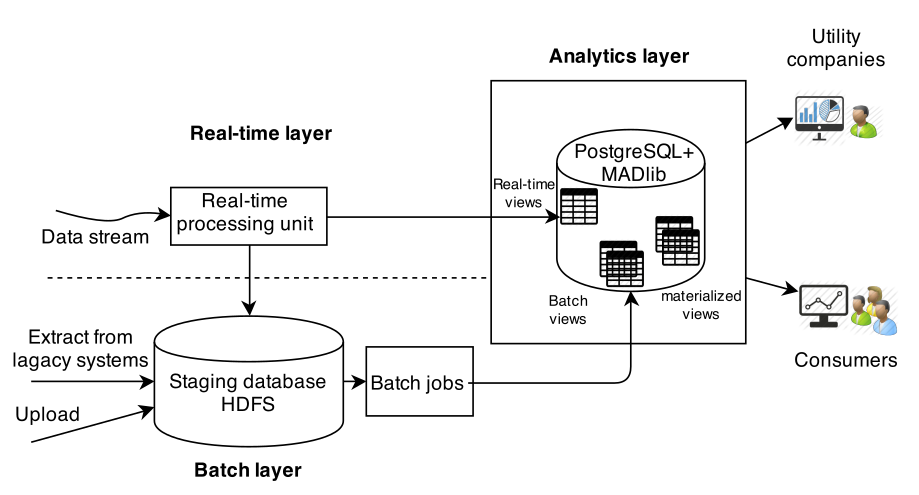
\includegraphics{img/smas_architecture.png}
\caption{Architektura systemu SMAS, źródło:
{[}\protect\hyperlink{ref-liu_smas_2015}{13}{]}}\label{fig:smas_architecture}
}
\end{figure}

Jak zaznaczono w pracy
{[}\protect\hyperlink{ref-molina-markham_private_2010}{14}{]}, poprzez
uzyskanie dostępu do danych z inteligentnego licznika można wywnioskować
odpowiedzi na wiele pytań dotyczących osobistych, potencjalnie głęboko
prywatnych, zachowań użytkowników. Podczas, gdy niektóre z tych
odpowiedzi mogą się wydawać nieszkodliwe, jak np. pora oglądania
telewizji, inne mogą być dość dotkliwe, jak np. obserwacja, że w domu
obecny jest noworodek.

Niektóre z odpowiedzi na potencjalnie delikatne pytania wyszczególniono
na \cref{fig:disturbing_answers} za
{[}\protect\hyperlink{ref-molina-markham_private_2010}{14}{]}.

\begin{figure}
\hypertarget{fig:disturbing_answers}{%
\centering
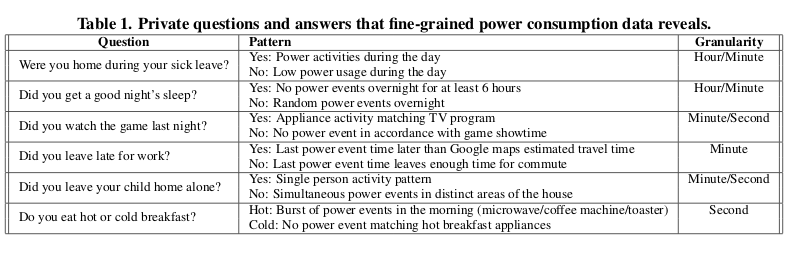
\includegraphics{img/disturbing_answers.png}
\caption{Wybrane potencjalnie delikatne pytania i wzorce wnioskowania o
odpowiedziach na nie, źródło:
{[}\protect\hyperlink{ref-molina-markham_private_2010}{14}{]}}\label{fig:disturbing_answers}
}
\end{figure}

\hypertarget{proces-dodawania-elastycznego-odbiorcy-do-puli-usux142ug-dsr}{%
\subsection{Proces dodawania elastycznego odbiorcy do puli usług
DSR}\label{proces-dodawania-elastycznego-odbiorcy-do-puli-usux142ug-dsr}}

Bieżący schemat procedury kwalifikacji elastycznego odbiorcy do programu
DSR przedstawia \cref{fig:certyfikacja}. Schemat pochodzi z prezentacji
aktualnych reguł aukcji DSR na polskim rynku energii elektrycznej.

\begin{figure}
\hypertarget{fig:certyfikacja}{%
\centering
\includegraphics{img/certyfikacja_ored_ogólnie.png}
\caption{Przebieg certyfikacji elastycznego odbiorcy, źródło:
{[}\protect\hyperlink{ref-socha_dsr_2018}{15}{]}}\label{fig:certyfikacja}
}
\end{figure}

W trakcie procesu certyfikacji, elastyczny odbiorca deklaruje kluczowe
parametry swojej oferty. Parametry te przedstawia \cref{fig:parametry}.

\begin{figure}
\hypertarget{fig:parametry}{%
\centering
\includegraphics{img/parametry_produktów_ored.png}
\caption{Parametry do podania przez Obiekt Redukcji w propozycji
sprzedaży, źródło:
{[}\protect\hyperlink{ref-socha_dsr_2018}{15}{]}}\label{fig:parametry}
}
\end{figure}

Proces przyjmowania odbiorcy do puli DSR w przypadku pomyślnego toku
zdarzeń kończy się przyznaniem certyfikatu. Przebieg tego procesu
ilustruje \cref{fig:certyfikacja_2}.

\begin{figure}
\hypertarget{fig:certyfikacja_2}{%
\centering
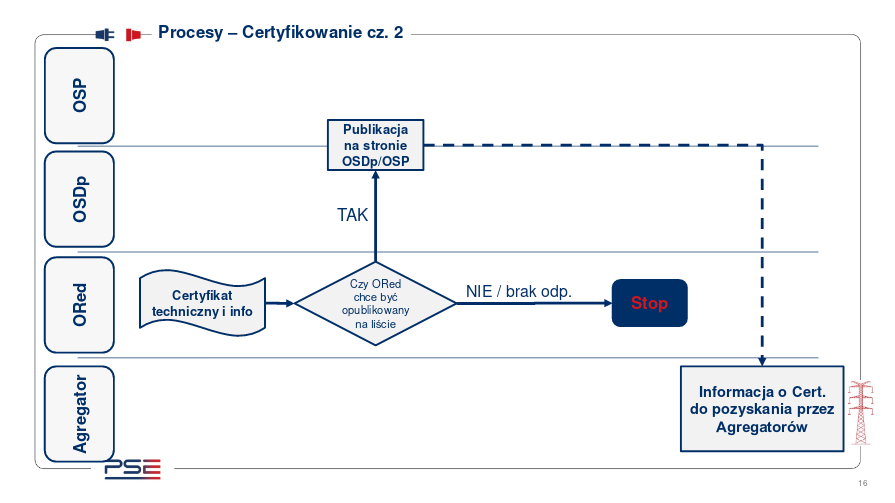
\includegraphics{img/certyfikacja_ored.png}
\caption{Procedura przyznania certyfikatu elastycznemu odbiorcy, źródło:
{[}\protect\hyperlink{ref-socha_dsr_2018}{15}{]}}\label{fig:certyfikacja_2}
}
\end{figure}

Propozycji zautomatyzowania tego procesu dostarcza praca
{[}\protect\hyperlink{ref-klos_market_2018}{16}{]}. Ujęto w niej
ilościowo procedurę przyjęcia elastycznego odbiorcy do programu DSR.
Proces przyjęcia odbiorcy polega na dołączeniu jego oferty do puli usług
branych pod uwagę.

Oferta każdego z odbiorców, wraz z jej konkretnymi parametrami:
wymiarem, ceną oraz jakością, nazywana jest dalej ``produktem''. Na
procedurę wyboru składają się następujące kroki:

\begin{enumerate}
\def\labelenumi{\arabic{enumi}.}
\tightlist
\item
  Wybranie najtańszego zestawu dostępnych produktów DSR Rozwiązanie
  szczególnego przypadku ``problemu plecakowego'' przy użyciu puli
  produktów oferowanych przez elastycznych odbiorców,
\item
  W razie niemożności skomponowania puli wystarczającej, wyznaczenie
  puli maksymalizującej uzyskaną moc, i na końcu
\item
  Wybranie i przetestowanie puli ostatecznie wybranych produktów.
\end{enumerate}

\hypertarget{problemy-1}{%
\section{Problemy}\label{problemy-1}}

Ponadto, pośród rozwiązań tej klasy na rynku energii nie ma rozwiązania,
które pozwalałoby na prosty wgląd do kodu źródłowego, przetestowanie go
w warunkach właściwych dla użytkowanego systemu przetwarzania danych czy
prostoą, samodzielną adaptację do własnych potrzeb.

\hypertarget{cel-pracy}{%
\chapter{Cel pracy}\label{cel-pracy}}

Celem tej pracy jest uproszczenie procesu certyfikacji elastycznych
odbiorców dla potrzeb programu DSR z perspektywy certyfikującego oraz
certyfikowanego.

\hypertarget{definicja-problemu}{%
\section{Definicja problemu}\label{definicja-problemu}}

Poszukiwana jest architektura do celów zautomatyzowanego profilowania
konsumentów pod kątem elastyczności
{[}\protect\hyperlink{ref-alahakoon_smart_2016}{17}{]}, uzupełniającego
dostępne rozwiązania automatycznego sterowania odbiornikami w systemie
DSR {[}\protect\hyperlink{ref-curtis_demand_2018}{7}{]}. Za podstawę
profilowania przyjmuje się funkcję indeksu elastyczności \(FI\) oraz
niepewność jej wyznaczenia.

\begin{figure}
\hypertarget{fig:stakeholders}{%
\centering
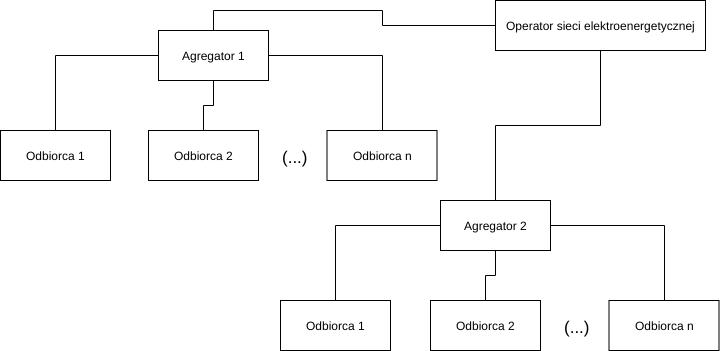
\includegraphics{img/aktorzy.png}
\caption{Relacje pomiędzy głównymi interesariuszami projektu,
opracowanie własne.}\label{fig:stakeholders}
}
\end{figure}

Z perspektywy interesariuszy, priorytetami projektu są następujące
aspekty:

\begin{itemize}
\tightlist
\item
  bezpieczeństwo danych użytkownika,
\item
  wiarygodność danych dostarczanych przez system zamawiającemu, oraz
\item
  wygoda interfejsów dla użytkownika i zamawiającego.
\end{itemize}

Zależności pomiędzy głównymi interesariuszami przedstawiono na
\cref{fig:stakeholders}. Charakterystyczną cechą architektury FMA jest
przechowywanie i przetwarzanie wrażliwych danych o odbiorcy przy użyciu
urządzeń zainstalowanych u niego samego. Do realizacji tego zadania
przewidziano opisywaną dalej kombinację elementów.

\hypertarget{podsumowanie}{%
\chapter{Podsumowanie}\label{podsumowanie}}

Celem tej pracy było przedstawienie architektury umożliwiającej
zautomatyzowaną ocenę elastyczności odbiorcy energii elektrycznej w
kontekście udziału w programie DSR.

Przedstawiona w tej pracy architektura spełnia postawione przez nią
zadanie, implementując ocenę elastyczności ze szczególnym uwzględnieniem
bezpieczeństwa wrażliwych danych o odbiorcy, wiarygodności rezultatów,
wygody dostępu do wyników pomiaru oraz łatwości dalszego rozwoju
systemu.

Charakterystyka architektury FMA sprawia, że odbiorca może w bardziej
zautomatyzowany sposób zrównoważyć koszty odbieranej energii zyskami z
tytułu modyfikowania profilu swego zapotrzebowania.

Warto zwrócić uwagę, iż opracowana architektura może być użyta do
szacowania energetycznej samowystarczalności zarówno pojedynczych
odbiorników, jak i budynków a nawet ich zespołów. Jak podają autorzy
przykładowych badań, zgrupowanie 700 gospodarstw domowych do celów
pomiaru ich zagregowanej elastyczności zgodnie ze wzorem \eqref{eq:fi},
pozwoliło na osiągnięcie niepewności pomiaru nie przekraczającej 10\%
{[}\protect\hyperlink{ref-wang_development_2018}{18}{]}.

\begin{equation} y = mx + b \label{eq:fi}\end{equation}

\hypertarget{wnioski}{%
\section{Wnioski}\label{wnioski}}

Zaprojektowanie rozwiązania odpowiadającego postawionym kryteriom
okazało się możliwe, a przygotowany prototyp potwierdził działanie
rozwiązania w zamierzony sposób.

\hypertarget{literatura}{%
\chapter*{Literatura}\label{literatura}}
\addcontentsline{toc}{chapter}{Literatura}

\setlength{\parindent}{0em}

\hypertarget{refs}{}
\begin{cslreferences}
\leavevmode\hypertarget{ref-finck_quantifying_2018}{}%
{[}1{]} C. Finck, R. Li, R. Kramer, and W. Zeiler, ``Quantifying demand
flexibility of power-to-heat and thermal energy storage in the control
of building heating systems,'' \emph{Applied Energy}, vol. 209, pp.
409--425, Jan. 2018, doi:
\href{https://doi.org/10.1016/j.apenergy.2017.11.036}{10.1016/j.apenergy.2017.11.036}.

\leavevmode\hypertarget{ref-junker_characterizing_2018}{}%
{[}2{]} R. G. Junker \emph{et al.}, ``Characterizing the energy
flexibility of buildings and districts,'' \emph{Applied Energy}, vol.
225, pp. 175--182, Sep. 2018, doi:
\href{https://doi.org/10.1016/j.apenergy.2018.05.037}{10.1016/j.apenergy.2018.05.037}.

\leavevmode\hypertarget{ref-leks_pare_2010}{}%
{[}3{]} M. Leks, ``Parę słów o architekturze korporacyjnej \textbar{}
ArchiReq \textbar{} Architektura korporacyjna w praktyce,'' May 23,
2010.
\url{http://archireq.pl/pl/pare-slow-o-architekturze-korporacyjnej/}
(accessed Jan. 14, 2019).

\leavevmode\hypertarget{ref-dolega_national_2018}{}%
{[}4{]} W. Dołęga, ``National grid electrical power infrastructure --
threats and challenges,'' \emph{Polityka Energetyczna}, vols. T. 21, z.
2, 2018, doi: \href{https://doi.org/10.24425/122769}{10.24425/122769}.

\leavevmode\hypertarget{ref-pap_pse_2015}{}%
{[}5{]} PAP, ``PSE: wprowadzenie stopni zasilania w sierpniu zapobiegło
blackoutowi,'' \emph{energianews}, Nov. 03, 2015.
\url{https://energia.rp.pl/energetyka-zawodowa/elektroenergetyka/10388-pse-wprowadzenie-stopni-zasilania-w-sierpniu-zapobieglo-blackoutowi}
(accessed Dec. 24, 2018).

\leavevmode\hypertarget{ref-ramchurn_putting_2012}{}%
{[}6{]} S. D. Ramchurn, P. Vytelingum, A. Rogers, and N. R. Jennings,
``Putting the 'smarts' into the smart grid: A grand challenge for
artificial intelligence,'' \emph{Communications of the ACM}, vol. 55,
no. 4, pp. 86--97, Jan. 2012, doi:
\href{https://doi.org/10.1145/2133806.2133825}{10.1145/2133806.2133825}.

\leavevmode\hypertarget{ref-curtis_demand_2018}{}%
{[}7{]} M. Curtis, J. Torriti, and S. T. Smith, ``Demand Side
Flexibility and Responsiveness: Moving Demand in Time Through
Technology,'' in \emph{Demanding Energy: Space, Time and Change}, A.
Hui, R. Day, and G. Walker, Eds. Cham: Springer International
Publishing, 2018, pp. 283--312.

\leavevmode\hypertarget{ref-lund_review_2015}{}%
{[}8{]} P. D. Lund, J. Lindgren, J. Mikkola, and J. Salpakari, ``Review
of energy system flexibility measures to enable high levels of variable
renewable electricity,'' \emph{Renewable and Sustainable Energy
Reviews}, vol. 45, pp. 785--807, May 2015, doi:
\href{https://doi.org/10.1016/j.rser.2015.01.057}{10.1016/j.rser.2015.01.057}.

\leavevmode\hypertarget{ref-kulkarni_perfect_2016}{}%
{[}9{]} S. Kulkarni, W. Randall, and D. Nowicki, ``The Perfect
Formula,'' \emph{Supply Chain Management Review}, vol. March, pp.
12--19, Mar. 2016.

\leavevmode\hypertarget{ref-lu_probabilistic_2018}{}%
{[}10{]} Z. Lu, H. Li, and Y. Qiao, ``Probabilistic Flexibility
Evaluation for Power System Planning Considering Its Association With
Renewable Power Curtailment,'' \emph{Power Systems, IEEE Transactions
on}, vol. 33, no. 3, pp. 3285--3295, 2018, doi:
\href{https://doi.org/10.1109/TPWRS.2018.2810091}{10.1109/TPWRS.2018.2810091}.

\leavevmode\hypertarget{ref-carroll_household_2018}{}%
{[}11{]} P. Carroll, T. Murphy, M. Hanley, D. Dempsey, and J. Dunne,
``Household Classification Using Smart Meter Data,'' \emph{Journal of
Official Statistics}, vol. 34, no. 1, pp. 1--25, Mar. 2018, doi:
\href{https://doi.org/10.1515/jos-2018-0001}{10.1515/jos-2018-0001}.

\leavevmode\hypertarget{ref-liu_smart_2016}{}%
{[}12{]} X. Liu, L. Golab, W. Golab, I. F. Ilyas, and S. Jin, ``Smart
Meter Data Analytics: Systems, Algorithms and Benchmarking,'' \emph{A C
M Transactions on Database Systems}, vol. 42, no. 1, 2016, doi:
\href{https://doi.org/10.1145/3004295}{10.1145/3004295}.

\leavevmode\hypertarget{ref-liu_smas_2015}{}%
{[}13{]} X. Liu, L. Golab, and I. F. Ilyas, ``SMAS: A smart meter data
analytics system,'' in \emph{2015 IEEE 31st International Conference on
Data Engineering}, Apr. 2015, pp. 1476--1479, doi:
\href{https://doi.org/10.1109/ICDE.2015.7113405}{10.1109/ICDE.2015.7113405}.

\leavevmode\hypertarget{ref-molina-markham_private_2010}{}%
{[}14{]} A. Molina-Markham, P. Shenoy, K. Fu, E. Cecchet, and D. Irwin,
``Private memoirs of a smart meter,'' in \emph{Proceedings of the 2nd
ACM Workshop on Embedded Sensing Systems for Energy-Efficiency in
Building - BuildSys '10}, 2010, p. 61, doi:
\href{https://doi.org/10.1145/1878431.1878446}{10.1145/1878431.1878446}.

\leavevmode\hypertarget{ref-socha_dsr_2018}{}%
{[}15{]} J. Socha, ``DSR Program Bieżący Uproszczony,'' \emph{Polskie
Sieci Elektroenergetyczne S.A.}, p. 26, Jul. 2018.

\leavevmode\hypertarget{ref-klos_market_2018}{}%
{[}16{]} M. Klos, M. Jakubek, and M. Krupa, ``On a Market Design of
Emergency DSR in Poland - Valuation and Optimal Acquisition of
Services,'' in \emph{2018 15th International Conference on the European
Energy Market (EEM)}, Jun. 2018, pp. 1--5, doi:
\href{https://doi.org/10.1109/EEM.2018.8469799}{10.1109/EEM.2018.8469799}.

\leavevmode\hypertarget{ref-alahakoon_smart_2016}{}%
{[}17{]} D. Alahakoon and X. Yu, ``Smart Electricity Meter Data
Intelligence for Future Energy Systems: A Survey,'' \emph{IEEE
Transactions on Industrial Informatics}, vol. 12, no. 1, pp. 425--436,
Feb. 2016, doi:
\href{https://doi.org/10.1109/TII.2015.2414355}{10.1109/TII.2015.2414355}.

\leavevmode\hypertarget{ref-wang_development_2018}{}%
{[}18{]} A. Wang, R. Li, and S. You, ``Development of a data driven
approach to explore the energy flexibility potential of building
clusters,'' \emph{Applied Energy}, vol. 232, pp. 89--100, Dec. 2018,
doi:
\href{https://doi.org/10.1016/j.apenergy.2018.09.187}{10.1016/j.apenergy.2018.09.187}.
\end{cslreferences}
